\chapter{Programação Estruturada}\label{cap_progest}

\hl{No paradigma de programação estruturada, o programa é organizado em blocos de códigos}. Cada bloco tem uma entrada de dados, um processamento (execução de uma tarefa) e produz uma saída.

\begin{figure}[H]
  \centering
  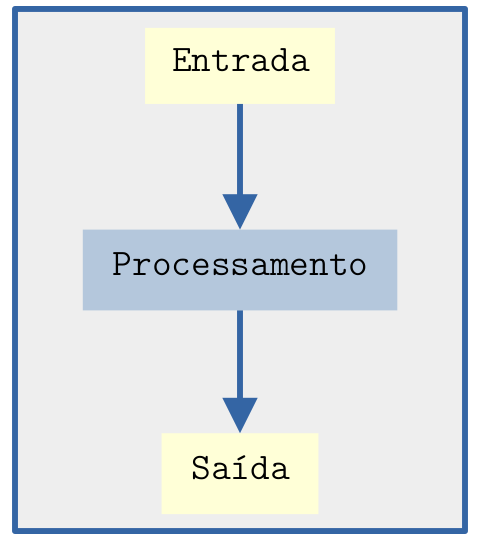
\includegraphics[width=1.5in]{./cap_progest/dados/fig_fg_bloco/fig.png}
  \caption{Bloco de processamento.}
  \label{cap_progest:fig:fg_bloco}
\end{figure}

Blocos podem ser colocados em sequência, selecionados com base em condições lógicas, iterados ou colocados dentro de outros blocos (sub-blocos).

\section{Estruturas de um Programa}\label{cap_progest_sec_est}

\hl{Para escrever qualquer programa, apenas três estruturas são necessárias: \emph{sequência}, \emph{seleção/ramificação} e \emph{iteração}}.

\subsection{Sequência}

A estrutura de \hl{\emph{sequência}} apenas significa que \hl{os blocos de programação são executados em sequência}. Ou seja, a execução de um bloco começa somente após a finalização do bloco anterior.

\begin{figure}[H]
  \centering
  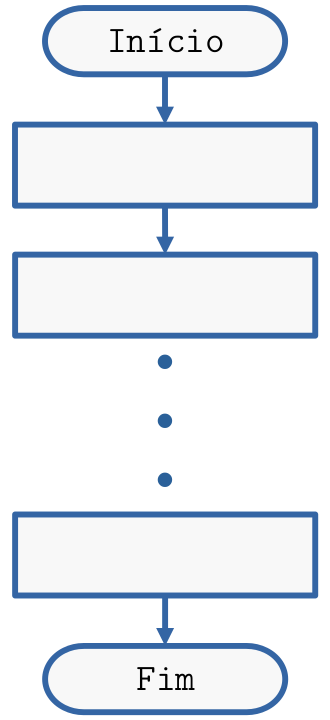
\includegraphics[width=2in]{./cap_progest/dados/fig_fg_sequencia/fig.png}
  \caption{Estrutura de sequência de blocos.}
  \label{cap_progest:fig:fg_sequencia}
\end{figure}

\begin{ex}
  O seguinte código computada a área do triângulo de base e altura informadas pela(o) usuária(o).

\begin{lstlisting}
#início

# bloco: entrada de dados
base = float(input('Digite a base:\n'))
altura = float(input('Digite a altura\n'))

# bloco: computação da área
area = base*altura/2

# bloco: saída de dados
print(f'Área = {area}')

#fim
\end{lstlisting}

O código acima está estruturado em três blocos. O primeiro bloco (linhas 3-5) processa a entrada de dados, seu término ocorre somente após a(o) usuária(o) digitar os valores da base e da altura. Na sequência, o bloco (linhas 7-8) faz a computação da área do triângulo e aloca o resultado na variável \lstinline+area+. No que este bloco termina seu processamento, é executado o último bloco (linhas 10-11), que imprime o resultado na tela.
\end{ex}

\subsection{Ramificação}

\hl{Estruturas de ramificação permitem a seleção de um ou mais blocos com base em condições lógicas}.

\begin{ex}\label{cap_progest_sec_est:ex:ramifica}
  O seguinte código lê um número inteiro digitado pela(o) usuária(o) e imprime uma mensagem no caso do número digitado ser par.

\begin{lstlisting}
#início

# entrada de dados
n = int(input('Digite um número inteiro:\n'))

# ramificação
if n%2 == 0:
  print(f'{n} é par.')

#término
\end{lstlisting}

Observamos que, no caso do número digitado não ser par, o programa termina sem nenhuma mensagem ser impressa. Esse é um exemplo de um bloco de ramificação, a instrução de ramificação (linha 7) testa a condição de \lstinline+n+ ser par. Somente no caso de ser verdadeiro, a instrução de impressão (linha 8) é executada. Após e impressão o programa é encerrado. No caso de \lstinline+n+ não ser par, o programa é encerrado sem que a instrução da linha 8 seja executada, i.e. a mensagem não é impressa.

\begin{figure}[H]
  \centering
  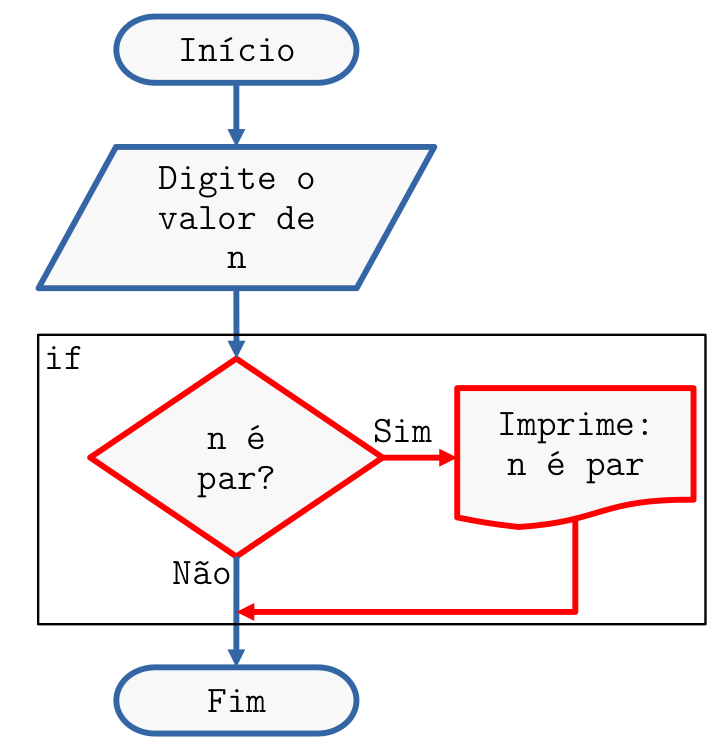
\includegraphics[width=2in]{./cap_progest/dados/fig_fg_ramifica/fig.png}
  \caption{Fluxograma de uma estrutura de ramificação.}
  \label{cap_progest:fig:fg_ramifica}
\end{figure}
  
\end{ex}

\begin{obs}[\hl{Indentação}]
  Na linguagem {\python}, a \emph{indentação} do código marca o início e o fim do bloco de código que pertence à instrução de ramificação. No Exemplo~\ref{cap_progest_sec_est:ex:ramifica}, o bloco selecionado pela instrução {\PYTHONif} é apenas a linha de código 8.
\end{obs}

\subsection{Repetição}

\hl{Instruções de repetição permitem que um mesmo bloco seja processado várias vezes em sequência}. Em {\python}, há duas instruções de repetição disponíveis: {\PYTHONfor} e {\PYTHONwhile}. 

\subsubsection{\texttt{for}}

A instrução \hl{{\PYTHONfor} permite que um bloco seja iterado para cada elemento de uma dada coleção de dados}.

\begin{ex}\label{cap_progest_sec_est:ex:for}
  O seguinte código testa a paridade de cada um dos elementos do conjunto $\{-3, -2, -1, 0, 1, 2, 3\}$.

\begin{lstlisting}
#início

# repetição for
for n in {-3, -2, -1, 0, 1, 2, 3}:
  res = (n%2 == 0)
  print(f'{n} é par? ', res)
    
#término
\end{lstlisting}

A instrução de repetição {\PYTHONfor} (linha 4), aloca em \lstinline+n+ um dos elementos do conjunto. Então, executa em sequência o bloco de comandos das linhas 5 e 6. De forma iterada, \lstinline+n+ recebe um novo elemento do conjunto e o bloco das linhas 5 e 6 é novamente executado. A repetição termina quando todos os elementos do conjunto já tiverem sido iterados. O código segue, então, para a linha 7. Não havendo mais instruções, o programa é encerrado.

\begin{figure}[H]
  \centering
  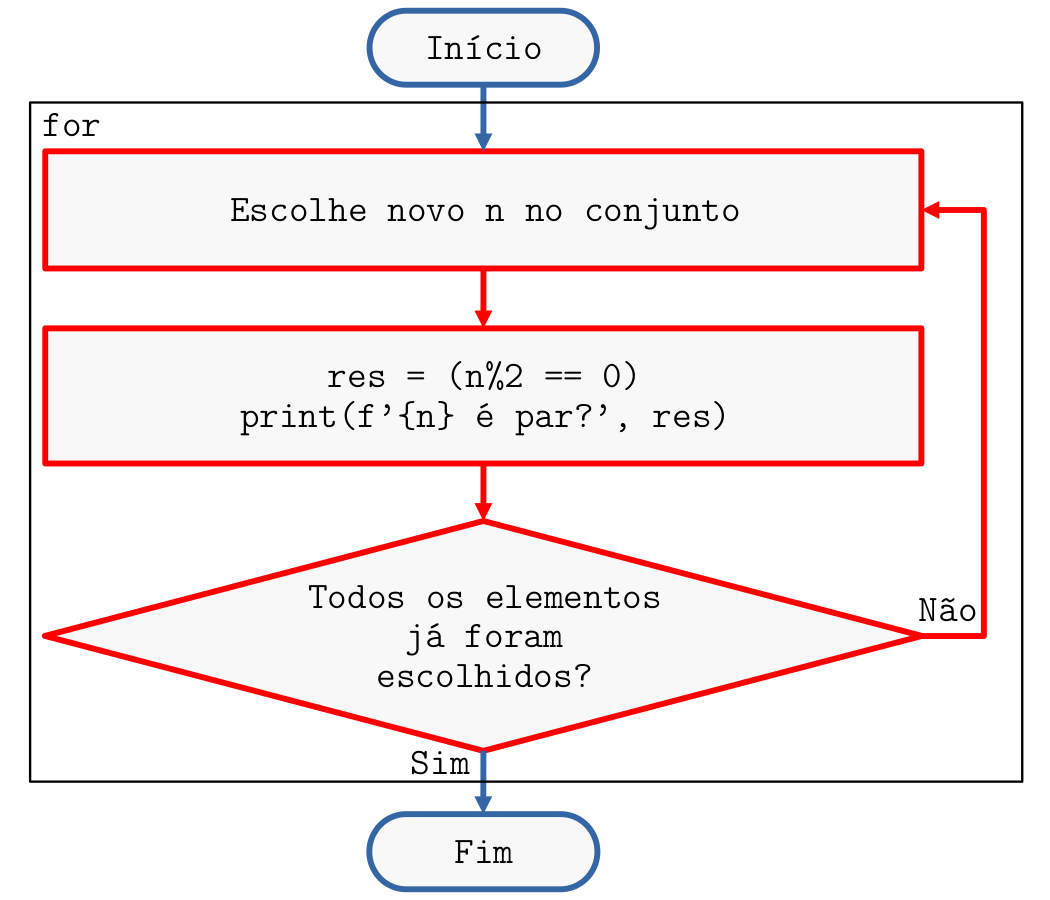
\includegraphics[width=2.75in]{./cap_progest/dados/fig_fg_for/fig.png}
  \caption{Fluxograma de uma estrutura de repetição do tipo {\PYTHONfor}.}
  \label{cap_progest_sec_est:fig:fg_for}
\end{figure}

Assim como no caso de uma instrução de ramificação, \hl{o bloco do {\PYTHONfor} é definido pela indentação do código}. Neste exemplo, o bloco são as linhas 5 e 6.
\end{ex}

\subsubsection{\texttt{while}}

A instrução \hl{{\PYTHONwhile} permite a repetição de um bloco enquanto uma dada condição lógica é satisfeita}.

\begin{ex}\label{cap_progest_sec_est:ex:while}
  O seguinte código testa a paridade dos números inteiros compreendidos de $-3$ a $3$.

\begin{lstlisting}
#início

n = -3

# repetição: while
while n <= 3:
  res = (n%2 == 0)
  print(f'{n} é par?', res)
  n += 1
    
#término
\end{lstlisting}

\begin{figure}[ht]
  \centering
  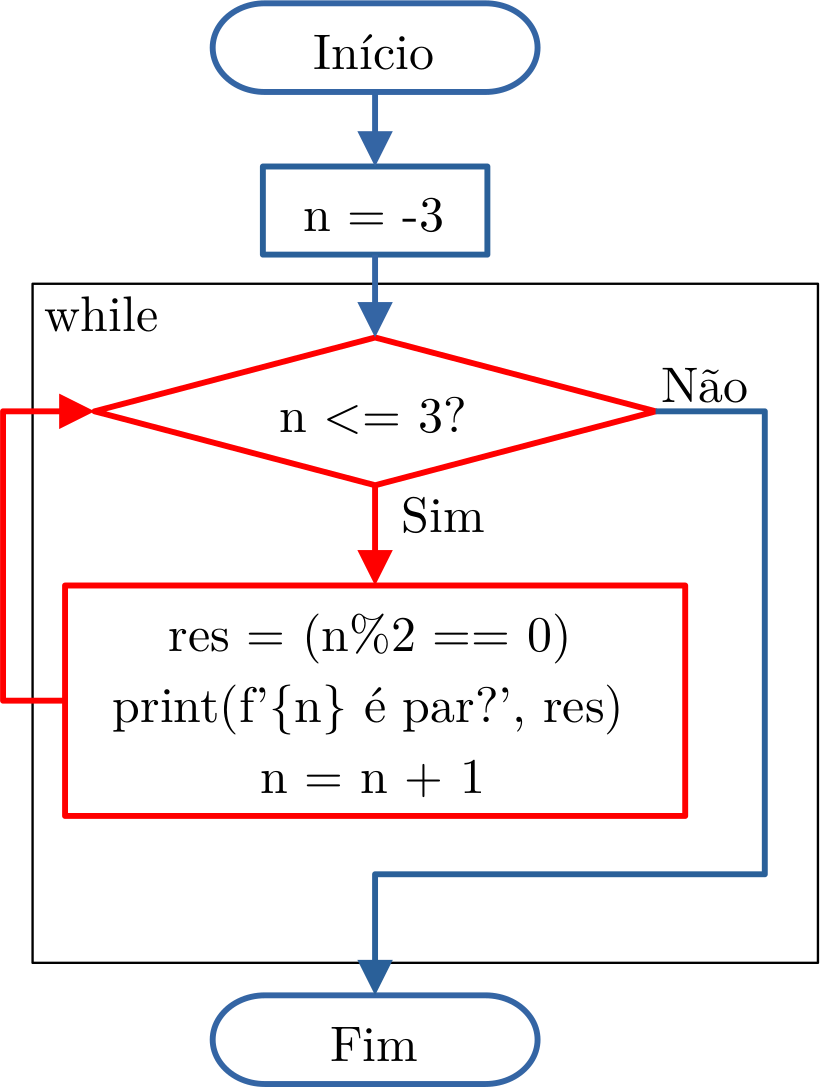
\includegraphics[width=2.5in]{./cap_progest/dados/fig_fg_while_ex/fig.png}
  \caption{Fluxograma da estrutura de repetição do tipo {\PYTHONwhile} para o Exemplo \ref{cap_progest_sec_est:ex:while}.}
  \label{cap_progest_sec_est:fig:fg_while_ex}
\end{figure}


A instrução de repetição {\PYTHONwhile} faz com que o bloco de processamento definido pelas linhas 7-9 seja executado de forma sequencial enquanto o valor de \texttt{n} for menor ou igual a 3. No caso dessa condição ser verdadeira, o bloco (linhas 7-9) é executado e, então a condição é novamente verificada. No caso da condição ser falsa, esse bloco não é executado e o código segue para a linha 10. Não havendo mais nenhuma instrução, o programa é encerrado.

Observamos que, neste exemplo, \hl{o bloco {\PYTHONwhile}} são as linhas 7-9, \hl{determinado pela indentação do código}.
\end{ex}

\subsection{Exercícios}

% exercícios de compreensão

\begin{exer}
  Complete as lacunas.
  \begin{enumerate}[a)]
    \item As seguintes estruturas são suficientes para escrever qualquer programa: \underline{\phantom{sequência}}, \underline{\phantom{seleção}} e \underline{\phantom{iteração}}.
    \item A estrutura de sequência significa que a execução de um bloco começa somente após a \underline{\phantom{finalização}} do bloco anterior.
    \item A estrutura de seleção permite a escolha de execução de um ou mais blocos com base em \underline{\phantom{condições lógicas}}.
    \item O bloco de código de uma instrução de repetição é determinado pela \underline{\phantom{indentação}} do código.
    \item Instruções de \underline{\phantom{repetição}} permitem que um mesmo bloco seja processado várias vezes de forma iterativa.
  \end{enumerate}
\end{exer}
\begin{resp}
  a) sequência, seleção e iteração. b) finalização. c) condições lógicas. d) indentação. e) repetição.
\end{resp}

\begin{exer}
  Complete as lacunas.
  \begin{enumerate}[a)]
    \item Uma estrutura de ramificação é implementada com a instrução \underline{\phantom{\texttt{if}}}.
    \item A instrução \underline{\phantom{\texttt{for}}} permite que um bloco seja iterado para cada elemento de uma coleção de dados iterável.
    \item A instrução \underline{\phantom{\texttt{while}}} permite a repetição de um bloco enquanto uma dada condição lógica é satisfeita.
  \end{enumerate}
\end{exer}
\begin{resp}
  a) \texttt{if}. b) \texttt{for}. c) \texttt{while}.
\end{resp}

% exercícios de programação

\begin{exer}
  Seja a reta de equação
  \begin{equation}
    y = ax + b.
  \end{equation}
  Assumindo $a=2$ e $b=-3$, o seguinte código foi desenvolvido para computar o ponto $x$ de interseção da desta reta com o eixo das abscissas.

\begin{lstlisting}
x = -b/2*a
a = 2
b = -3
print(x)
\end{lstlisting}

Identifique e explique os erros desse código. Então, apresente uma versão corrigida.
\end{exer}
\begin{resp}

\begin{lstlisting}
a = 2
b = -3
x = -b/a
print(x)
\end{lstlisting}

\end{resp}

\begin{exer}\label{cap_progest_sec_est:exer:ramifica_reta}
  Seja a reta de equação
  \begin{equation}
    y = ax + b.
  \end{equation}
  Faça um fluxograma de um programa em que a(o) usuária(o) entra com os valores de $a$ e $b$. No caso de $a\neq 0$, o programa computa e imprime o ponto $x$ da interseção dessa reta com o eixo das abscissas.
\end{exer}
\begin{resp}

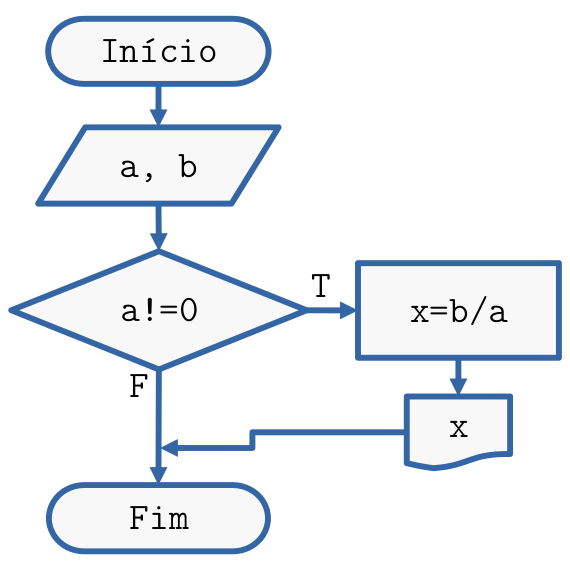
\includegraphics[width=1.5in]{cap_progest/dados/fig_exer_ramifica_reta/fig.png}
  
\end{resp}

\begin{exer}
  Implemente o código referente ao fluxograma criado no Exercício~\exerref{cap_progest_sec_est:exer:ramifica_reta}.
\end{exer}
\begin{resp}

\begin{lstlisting}
a = float(input('Digite o valor de a:\n'))
b = float(input('Digite o valor de b:\n'))
if (a != 0):
  x = -b/(2*a)
  print(f'Ponto de interseção com o eixo x = {x}')
\end{lstlisting}

\end{resp}

\begin{exer}\label{cap_progest_sec_est:exer:for}
  Faça o fluxograma de um programa que usa de um bloco de repetição {\PYTHONfor} para percorrer o conjunto
  \begin{equation}
    A = \{-4, -3, -2, -1, 0, 1, 2, 3, 4\}.
  \end{equation}
  A cada iteração, o programa imprime {\PYTHONTrue} ou {\PYTHONFalse} conforme o elemento seja ímpar ou não.
\end{exer}
\begin{resp}
  
  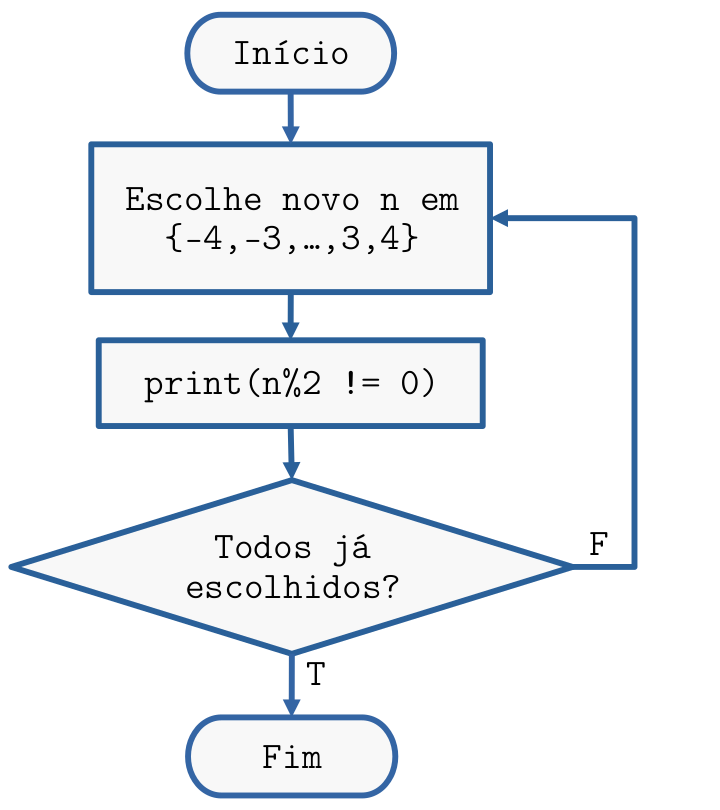
\includegraphics[width=3in]{cap_progest/dados/fig_exer_for/fig.png}

\end{resp}

\begin{exer}
  Implemente o código referente ao fluxograma criado no Exercício~\exerref{cap_progest_sec_est:exer:for}.
\end{exer}
\begin{resp}

\begin{lstlisting}
A = {-4, -3, -2, -1, \
     0, 1, 2, 3, 4}
for x in A:
  res = (x % 2 != 0)
  print(f'{x} é ímpar? {res}')
\end{lstlisting}

\end{resp}

\begin{exer}\label{cap_progest_sec_est:exer:while}
  Faça um fluxograma análogo ao do Exercício~\exerref{cap_progest_sec_est:exer:for} que use a instrução de repetição {\PYTHONwhile} no lugar de {\PYTHONfor}.
\end{exer}
\begin{resp}

  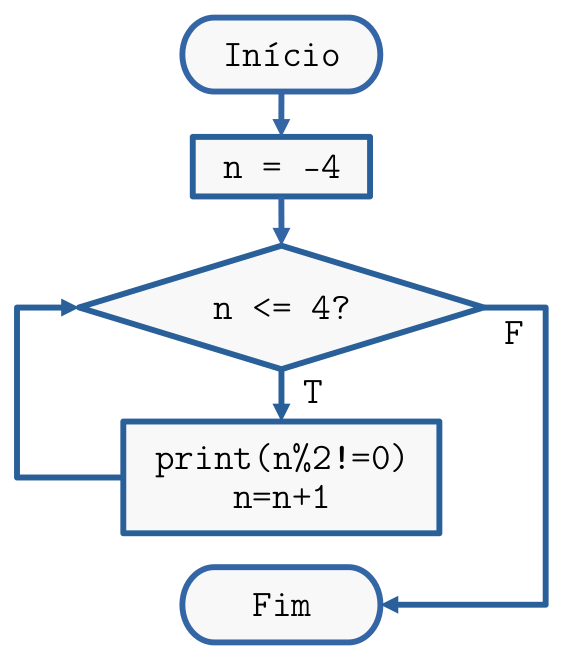
\includegraphics[width=2in]{cap_progest/dados/fig_exer_while/fig.png}

\end{resp}

\begin{exer}
  Implemente um código referente ao fluxograma criado no Exercício~\exerref{cap_progest_sec_est:exer:while}.
\end{exer}
\begin{resp}

\begin{lstlisting}
A = {-4, -3, -2, -1, \
     0, 1, 2, 3, 4}
n = -4
while (n <= 4):
  res = (n % 2 != 0)
  print(f'{n} é ímpar? {res}')
  n += 1
\end{lstlisting}

\end{resp}

\ifisbook
\subsubsection{Respostas}
\shipoutAnswer
\fi


\section{Instruções de Ramificação}\label{cap_progest_sec_ramifica}

\hl{Instruções de ramificação permitem a seleção de blocos de programação com base em condições lógicas}.

\subsection{Instrução \texttt{if}}

\hl{A instrução de ramificação {\PYTHONif} permite a seleção de um bloco de programação com base em uma condição lógica}.

\begin{figure}[H]
  \centering
  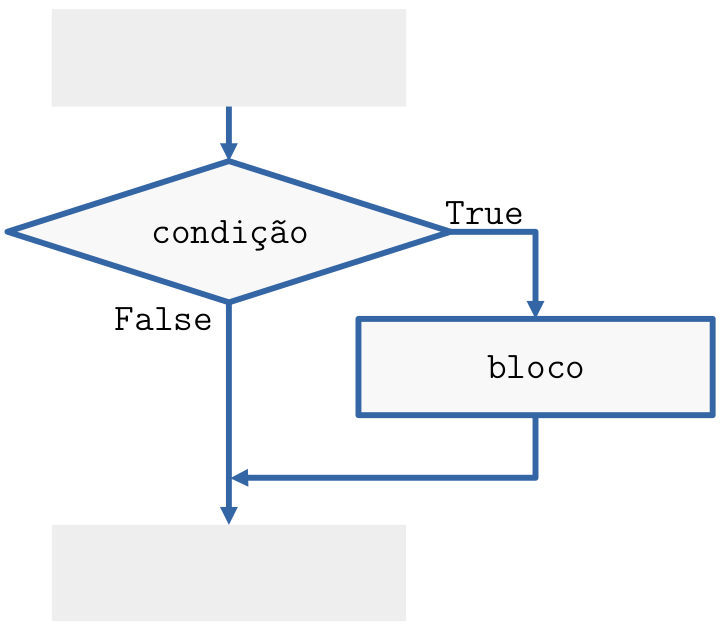
\includegraphics[width=2.25in]{./cap_progest/dados/fig_fg_if/fig.png}
  \caption{Fluxograma de uma ramificação {\PYTHONif}.}
  \label{cap_progest_sec_ramifica:fig:fg_if}
\end{figure}

Em {\python}, a \hl{instrução {\PYTHONif}} tem a seguinte \hl{sintaxe}:

\begin{lstlisting}
bloco_anterior
if condição:
  bloco_0
bloco_posterior
\end{lstlisting}

Se a {\lstinline+condição+} é verdadeira ({\PYTHONTrue}), o bloco (linha 3) é executado. Caso contrário, este bloco não é executado e o fluxo de processamento salta da linha 2 para a linha 6. O bloco selecionado pela instrução {\PYTHONif} é determinado pela indentação do código.

\begin{ex}\label{cap_progest_sec_ramifica:ex:bhaskara_if}
  Seja o polinômio de segundo grau
  \begin{equation}
    p(x) = ax^2 + bx + c.
  \end{equation}
  No caso de existirem, o seguinte código computa as raízes distintas de $p(x)$ para os coeficientes informados pela(o) usuária(o).

\begin{lstlisting}
# entrada de dados
a = float(input('Digite o valor de a:\n'))
b = float(input('Digite o valor de b:\n'))
c = float(input('Digite o valor de c:\n'))

# discriminante
delta = b**2 - 4*a*c

# raízes
if delta > 0:
  # raízes distintas
  x1 = (-b - delta**0.5)/(2*a)
  x2 = (-b + delta**0.5)/(2*a)
  print(f'x_1 = {x1}')
  print(f'x_2 = {x2}')
\end{lstlisting}

\end{ex}

\subsubsection{Escopo de Variáveis}

O \hlemph{escopo} de uma variável é a região em que ela permanece alocada. \hl{O escopo de variáveis alocadas fora do bloco {\PYTHONif} inclui este bloco, mas variáveis alocadas no bloco {\PYTHONif} não permanecem alocadas fora deste}.

\begin{ex}
  No Exemplo~\ref{cap_progest_sec_ramifica:ex:bhaskara_if}, o escopo da variável \lstinline+delta+ inicia-se na linha 7 e permanece válido ao longo do resto do programa. Já, o escopo da variável \lstinline+x1+ compreende somente as linhas 12-15 e, análogo para a variável \lstinline+x2+. 
\end{ex}

\subsection{Instrução \texttt{if-else}}

A instrução \hl{\texttt{if-else} permite a escolha de um bloco ou outro, exclusivamente, com base em uma condição lógica}.

\begin{figure}[H]
  \centering
  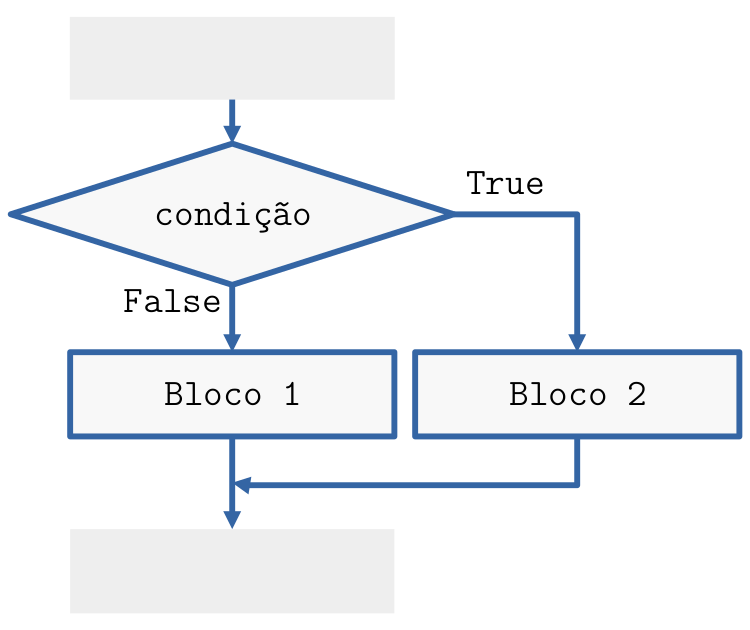
\includegraphics[width=2.25in]{./cap_progest/dados/fig_fg_else/fig.png}
  \caption{Fluxograma de uma ramificação \lstinline+if-else+.}
  \label{cap_progest_sec_ramifica:fig:fg_else}
\end{figure}

Em {\python}, a instrução \lstinline+if-else+ tem a seguinte sintaxe:

\begin{lstlisting}
bloco_anterior
if condição:
  bloco_0
else:
  bloco_1
bloco_posterior
\end{lstlisting}

Se a {\lstinline+condição+} for verdadeira ({\PYTHONTrue}) o {\lstinline+bloco 0+} é executado, senão o {\lstinline+bloco 1+} é executado.

\begin{ex}
  Seja o polinômio de segundo grau
  \begin{equation}
    p(x) = ax^2 + bx + c.
  \end{equation}
  Se existirem, o seguinte código computa as raízes reais do polinômio, senão imprime mensagem informado que elas não são reais.

\begin{lstlisting}
# entrada de dados
a = float(input('Digite o valor de a:\n'))
b = float(input('Digite o valor de b:\n'))
c = float(input('Digite o valor de c:\n'))

# discriminante
delta = b**2 - 4*a*c

# raízes
if delta >= 0:
  x1 = (-b - delta**0.5)/(2*a)
  x2 = (-b + delta**0.5)/(2*a)
  print(f'x_1 = {x1}')
  print(f'x_2 = {x2}')
else:
  print('Não tem raízes reais.')
\end{lstlisting}

\end{ex}

\subsubsection{Instrução \lstinline+if-else+ em Linha}

Por praticidade, {\python} também tem a sintaxe \lstinline+if-else+ em linha:

\begin{lstlisting}
x = valor if True else outro_valor
\end{lstlisting}

\begin{ex}
  O valor absoluto de um número real $x$ é
  \begin{equation}
    |x| := \left\{
      \begin{array}{ll}
        x &, x\geq 0,\\
        -x &, x<0
      \end{array}
    \right.
  \end{equation}
  O seguinte código, computa o valor absoluto\endnote{{\python} tem a função {\PYTHONabs} para computar o valor absoluto de um número.} de um número dado por usuária(o).
  
\begin{lstlisting}
x = float(input('Digite o valor de x:\n'))
abs_x = x if x>=0 else -x
print(f'|x| = {abs_x}')
\end{lstlisting}

\end{ex}

\subsection{Instrução \texttt{if-elif}}

\hl{A instrução \texttt{if-elif} permite a seleção condicional de blocos, sem impor a necessidade da execução de um deles}.

\begin{figure}[H]
  \centering
  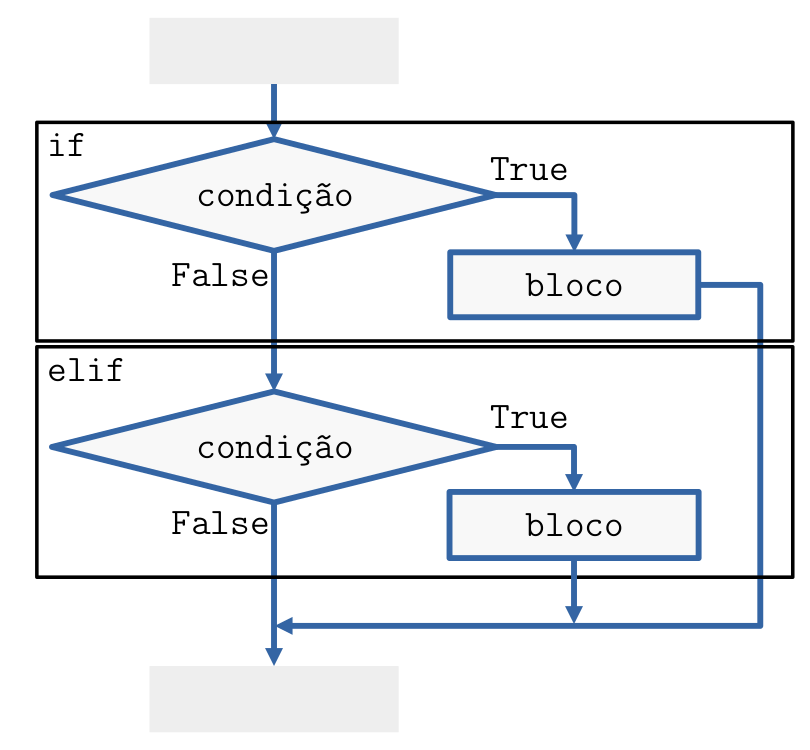
\includegraphics[width=2.5in]{./cap_progest/dados/fig_fg_elif/fig.png}
  \caption{Fluxograma de uma ramificação \lstinline+if-elif+.}
  \label{cap_progest_sec_ramifica:fig:fg_elif}
\end{figure}

Em {\python}, a instrução \lstinline+if-elif+ tem a seguinte sintaxe:

\begin{lstlisting}
bloco_anterior
if condição_0:
  bloco_0
elif condição 1:
  bloco_1
bloco posterior
\end{lstlisting}

Se a \lstinline+condição_0+ for verdadeira ({\PYTHONTrue}), o \lstinline+bloco_0+ é executado. Senão, se a \lstinline+condição_1+ for verdadeira ({\PYTHONTrue}) o \lstinline+bloco_1+ é executado. No caso de ambas as condições serem falsas ({\PYTHONFalse}), os blocos \lstinline+bloco_0+ e \lstinline+bloco_1+ não são executados e o fluxo de processamento segue a partir da linha 6.

\begin{ex}
  Seja o polinômio de segundo grau
  \begin{equation}
    p(x) = ax^2 + bx + c.
  \end{equation}
  Conforme o caso, o seguinte código computa a raiz dupla do polinômio ou suas raízes reais distintas, a partir dos coeficientes informados pela(o) usuária(o).

\begin{lstlisting}
# entrada de dados
a = float(input('Digite o valor de a:\n'))
b = float(input('Digite o valor de b:\n'))
c = float(input('Digite o valor de c:\n'))

# discriminante
delta = b**2 - 4*a*c

# raízes
if delta > 0:
  x1 = (-b - delta**0.5)/(2*a)
  x2 = (-b + delta**0.5)/(2*a)
  print('Raízes reais distintas:')
  print(f'x_1 = {x1}')
  print(f'x_2 = {x2}')
elif delta == 0:
  print('Raiz dupla:')
  x = -b/(2*a)
  print(f'x_1 = x_2 = {x}')
\end{lstlisting}

\end{ex}

\subsection{Instrução \texttt{if-elif-else}}

A instrução \lstinline+if-elif-else+ permite a seleção condicional de blocos, sendo que ao menos um bloco será executado. Em {\python}, sua sintaxe é:

\begin{lstlisting}
bloco_anterior
if condição_0:
  bloco_0
elif condição_1:
  bloco_1
else:
  bloco_2
bloco posterior
\end{lstlisting}

Se a \lstinline+condição_0+ for verdadeira ({\PYTHONTrue}), então o \lstinline+bloco_0+ é executado. Senão, se a \lstinline+condição_1+ for verdadeira ({\PYTHONTrue}), então o \lstinline+bloco_1+ é executado. Senão, o \lstinline+bloco_2+ é executado.

\begin{ex}
  Seja o polinômio de segundo grau
  \begin{equation}
    p(x) = ax^2 + bx + c.
  \end{equation}
  Conforme o caso (raízes reais distintas, raiz dupla ou raízes complexas), o seguinte código computa as raízes desse polinômio, a partir dos coeficientes informados pela(o) usuária(o).

\begin{lstlisting}
# entrada de dados
a = float(input('Digite o valor de a:\n'))
b = float(input('Digite o valor de b:\n'))
c = float(input('Digite o valor de c:\n'))

# discriminante
delta = b**2 - 4*a*c

# raízes
if delta > 0:
  # raízes distintas
  x1 = (-b - delta**0.5)/(2*a)
  x2 = (-b + delta**0.5)/(2*a)
  print('Raízes reais distintas:')
  print(f'x_1 = {x1}')
  print(f'x_2 = {x2}')
elif delta == 0:
  # raiz dupla
  x = -b/(2*a)
  print('Raiz dupla:')
  print(f'x_1 = x_2 = {x}')
else:
  # raízes complexas
  # parte real
  rea = -b/(2*a)
  # parte imaginária
  img = (-delta)**0.5/(2*a)
  x1 = rea - img*1j
  x2 = rea + img*1j
  print('Raízes complexas:')
  print(f'x_1 = {x1}')
  print(f'x_2 = {x2}')
\end{lstlisting}

\end{ex}

\subsection{Múltiplos Casos}

\hl{Pode-se encadear instruções \texttt{if-elif-elif-...-elif[-else]} para a seleção condicional entre múltiplos blocos}.

\begin{ex}
  Sejam as circunferências de equações:
  \begin{align}
    & c_1: (x-a_1)^2 + (y-b_1)^2 = r_1, \\
    & c_2: (x-a_1)^2 + (y-b_1)^2 = r_2.
  \end{align}
  Conforme entradas dadas por usuária(o), o seguinte código informa se um dado ponto $(x, y)$ pertence: à interseção dos discos determinados por $c_1$ e $c_2$, apenas ao disco determinado por $c_1$, apenas ao disco determinado por $c_2$ ou a nenhum desses discos.

\begin{lstlisting}
# entrada de dados
print('c1: (x-a1)**2 + (y-b1)**2 = r1')
a1 = float(input('Digite o valor de a1:\n'))
b1 = float(input('Digite o valor de b1:\n'))
r1 = float(input('Digite o valor de r1:\n'))
print('c2: (x-a2)**2 + (y-b2)**2 = r1')
a2 = float(input('Digite o valor de a2:\n'))
b2 = float(input('Digite o valor de b2:\n'))
r2 = float(input('Digite o valor de r2:\n'))
print('Ponto de interesse (x,y).')
x = float(input('Digite o valor de x:\n'))
y = float(input('Digite o valor de y:\n'))

# pertence ao disco c1?
c1 = (x-a1)**2 + (y-b1)**2 <= r1
# pertence ao disco c2?
c2 = (x-a2)**2 + (y-b2)**2 <= r2

# imprime resultado
if c1 and c2:
  print(f'({x}, {y}) pertence à interseção dos discos.')
elif c1:
  print(f'({x},{y}) pertence ao disco c1.')
elif c2:
  print(f'({x},{y}) pertence ao disco c2.')
else:
  print(f'({x},{y}) não pertence aos discos.')
\end{lstlisting}

\end{ex}


\subsection{Exercícios}

% exercícios de comprensão

\begin{exer}
  Complete as lacunas.
  \begin{enumerate}[a)]
    % a)
    \item Instruções de ramificação permitem a \underline{\phantom{seleção}} de blocos códigos com base em condições lógicas.
    % b)
    \item Uma instrução \underline{\phantom{{\PYTHONif}}} permite a seleção de um bloco de código com base em uma condição \underline{\phantom{lógica}}.
    % c)
    \item O \underline{\phantom{escopo}} de uma variável é a região em que ela permanece alocada.
    % d)
    \item Uma instrução \underline{\phantom{\texttt{else}}} indica a seleção de um bloco de código com base na negação da condição de seleção do bloco imediatamente anterior.
    % e)
    \item Uma instrução \texttt{elif} permite impor uma \underline{\phantom{condição lógica}} adicional para a seleção de um bloco de código com base na negação da condição de seleção do bloco imediatamente anterior.
  \end{enumerate}
\end{exer}
\begin{resp}
  a) seleção; b) lógica; c) escopo; d) \texttt{else}; e) condição lógica
\end{resp}

% exercícios de programação

\begin{exer}
  Seja a equação de reta
  \begin{equation}
    ax + b = 0.
  \end{equation}
  Dados coeficientes $a \neq 0$ e $b$ informados por usuária(o), crie um código que imprime o ponto de interseção dessa reta com o eixo das abscissas. O código não deve tentar computar o ponto no caso de $a=0$. 
\end{exer}
\begin{resp}

\begin{lstlisting}
# entrada de dados
a = float(input('Digite o valor de a:\n'))
b = float(input('Digite o valor de b:\n'))

# computação
if a != 0:
  x = -b/a
  y = a*x + b
  print(f'Intercepta eixo-x em: ({x}, {y}).')
\end{lstlisting}

\end{resp}

\begin{exer}
  Considere o seguinte código.

\begin{lstlisting}
n = int(input('Digite um número inteiro:\n')
if n % 2 == 0:
  m = 1
n = n + m
print(n)
\end{lstlisting}

A ideia é que, se $n$ for ímpar, o código imprime $n$, caso contrário, imprime $n+1$. Este código contém erro. Identifique e explique-o, então proponha uma versão funcional.
\end{exer}
\begin{resp}

\begin{lstlisting}
n = int(input('Digite um número inteiro:\n')
m = 0
if n % 2 == 0:
  m = 1
n = n + m
print(n)
\end{lstlisting}

\end{resp}

\begin{exer}
  Considere o seguinte algoritmo/pseudocódigo para verificar se um dado número inteiro $n$ é par ou ímpar.

\ifisbook
\newpage
\fi
\begin{itemize}\setlength\itemsep{0em}
\item[0.] Início.
\item[1.] Usuária(o) informa o valor inteiro $n$.
\item[2.] Se o resto da divisão de $n$ por $2$ for igual a zero, então faça:
  \begin{itemize}\setlength\itemsep{0em}
  \item[2.1.] Imprime a mensagem: ``$n$ é par.''.
  \end{itemize}
\item[3.] Senão, faça:
  \begin{itemize}\setlength\itemsep{0em}
  \item[3.1] Imprime a mensagem: ``$n$ é ímpar''. 
  \end{itemize}
\item[4.] Fim.
\end{itemize}
Faça um fluxograma para esse algoritmo e implemente-o.
\end{exer}

\begin{exer}
  Considere a equação da circunferência
  \begin{equation}
    c: (x-a)^2 + (y-b)^2 = r^2.
  \end{equation}
  Com dados informados por usuária(o), desenvolva um código que informe se um dado ponto $(x, y)$ pertence ou não ao disco determinado por $c$.
\end{exer}
\begin{resp}

\begin{lstlisting}
# entrada de dados
print('Circunferência c:')
a = float(input('Digite o valor de a:\n'))
b = float(input('Digite o valor de b:\n'))
r = float(input('Digite o valor de r:\n'))
print('Ponto (x, y):')
x = float(input('Digite o valor de x:\n'))
y = float(input('Digite o valor de y:\n'))

# resultado
if (x-a)**2 + (y-b)**2 <= r**2:
  print(f'({x}, {y}) pertence ao disco.')
else:
  print(f'({x}, {y}) não pertence ao disco.')
\end{lstlisting}

\end{resp}

\begin{exer}\label{cap_progest_sec_ramifica:exer:intercep_retas}
  Sejam informadas por usuária(o) os coeficientes das retas
  \begin{align}
    & r_1: a_1x + b_1 = 0, \\
    & r_2: a_2x + b_2 = 0.
  \end{align}
  Crie um código que informe se as retas são paralelas. Caso contrário, o código imprime o ponto de interseção delas.
\end{exer}
\begin{resp}

\begin{lstlisting}
# entrada de dados
print('r1: a1*x + b1 = 0')
a1 = float(input('Digite o valor de a1:\n'))
b1 = float(input('Digite o valor de b1:\n'))
print('r2: a2*x + b2 = 0')
a2 = float(input('Digite o valor de a2:\n'))
b2 = float(input('Digite o valor de b2:\n'))

# resultado
if a1 == a2:
  print('r1 // r2')
else:
  x = (b1-b2)/(a2-a1)
  y = a1*x + b1
  print('Ponto de interseção: ({x}, {y}).')
\end{lstlisting}

\end{resp}

\begin{exer}
  Refaça o código do Exercício~\exerref{cap_progest_sec_ramifica:exer:intercep_retas} de forma a incluir o caso em que as retas sejam coincidentes. Ou seja, o código deve informar os seguintes casos: retas paralelas não coincidentes, retas coincidentes ou, caso contrário, ponto de interseção das retas.
\end{exer}
\begin{resp}

\begin{lstlisting}
# entrada de dados
print('r1: a1*x + b1 = 0')
a1 = float(input('Digite o valor de a1:\n'))
b1 = float(input('Digite o valor de b1:\n'))
print('r2: a2*x + b2 = 0')
a2 = float(input('Digite o valor de a2:\n'))
b2 = float(input('Digite o valor de b2:\n'))

# resultado
if a1 == a2:
  if (b1 == b2):
    print('r1 = r2')
  else:
    print('r1 // r2 e r1 != r2')
else:
  x = (b1-b2)/(a2-a1)
  y = a1*x + b1
  print('Ponto de interseção: ({x}, {y}).')
\end{lstlisting}

\end{resp}

\begin{exer}
  Sejam a parábola de equação
  \begin{equation}
    a_1x^2 + a_2x + a_3 = 0
  \end{equation}
  e a reta
  \begin{equation}
    b_1x + b_2 = 0.
  \end{equation}
  Conforme os coeficientes dados por usuária(o), desenvolva um código que imprime o(s) ponto(s) de interseção da reta com a parábola. O código deve avisar os casos em que: há apenas um ponto, há dois pontos ou não há ponto de interseção.
\end{exer}
\begin{resp}

\begin{lstlisting}
# entrada de dados
print('Coeficientes da parábola')
print('a1*x**2 + a2*x + a3 = 0')
a1 = float(input('Digite o valor de a1:\n'))
a2 = float(input('Digite o valor de a2:\n'))
a2 = float(input('Digite o valor de a3:\n'))

print('Coeficientes da reta')
print('b1*x + b2 = 0')
b1 = float(input('Digite o valor de b1:\n'))
b2 = float(input('Digite o valor de b2:\n'))

# discriminante da equação
# a1*x**2 + (a2-b1)*x + (a3-b2) = 0
delta = (a2-b1)**2 - 4*a1*(a3-b2)

# ponto(s) de interseção
if delta == 0:
  x = (b1-a2)/(2*a1)
  y = b1*x + b2
  print('Ponto de interseção:')
  print(f'({x}, {y})')
elif delta > 0:
  x1 = ((b1-a2) - delta**2)/(2*a1)
  y1 = b1*x1 + b2
  x2 = ((b1-a2) + delta**2)/(2*a1)
  y2 = b1*x2 + b2
  print('Pontos de interseção:')
  print(f'({x1}, {y1}), ({x2}, {y2})')
else:
  print('Não há ponto de interseção.')
\end{lstlisting}

\end{resp}

\begin{exer}
  Com dados informados por usuária(o), sejam as circunferências de equações
  \begin{align}
    & c_1: (x-a_1)^2 + (y-b_1)^2 = r_1^2, \\
    & c_2: (x-a_2)^2 + (y-b_2)^2 = r_2^2.
  \end{align}
  Desenvolva um código que informe a(o) usuária(o) dos seguintes casos: $c_1$ e $c_2$ são coincidentes, $c_1\cap c_2$ tem dois pontos, $c_1\cap c_2$ tem somente um ponto, $c_1\cap c_2 = \emptyset$.
\end{exer}
\begin{resp}

\begin{lstlisting}
# entrada de dados
print('c1: (x-a1)**2 + (y-b1)**2 = r1**2')
a1 = float(input('Digite o valor de a1:\n'))
b1 = float(input('Digite o valor de b1:\n'))
r1 = float(input('Digite o valor de r1:\n'))
print('c2: (x-a2)**2 + (y-b2)**2 = r2**2')
a2 = float(input('Digite o valor de a2:\n'))
b2 = float(input('Digite o valor de b2:\n'))
r2 = float(input('Digite o valor de r2:\n'))

# verificações
if a1==a2 and b1==b2 and r1==r2:
  print('c1 = c2')
else:
  # distância entre os centros
  dist = ((a2-a1)**2 + (b2-b1)**2)**0.5
  if (abs(dist - (r1+r2)) < 1e-15):
    print('c1 & c2 têm um único ponto de interseção.')
  elif (dist < r1+r2):
    print('c1 & c2 têm dois pontos de interseção.')
  else:
    print('c1 & c2 não tem ponto de interseção.')
\end{lstlisting}

\end{resp}

\begin{exer}
  Crie uma calculadora simples. A(o) usuária(o) entra com dois números decimais \lstinline+x+ e \lstinline+y+ e uma das seguintes operações: \lstinline!+!, \lstinline+-+, \lstinline+*+ ou \lstinline+/+. Então, o código imprime o resultado da operação.
\end{exer}
\begin{resp}

\begin{lstlisting}
# entrada de dados
x = float(input('Digite o valor de x:\n'))
op = input('Digite uma das operações +, -, * ou /:\n')
y = float(input('Digite o valor de y:\n'))

# calcula
if op == '+':
  print(f'{x} ' + op + f' {y} = {x+y}')
elif op == '-':
  print(f'{x} ' + op + f' {y} = {x-y}')
elif op == '*':
  print(f'{x} ' + op + f' {y} = {x*y}')
elif op == '/':
  print(f'{x} ' + op + f' {y} = {x/y}')
else:
  print('Desculpa, não entendi!')
\end{lstlisting}

\end{resp}

\begin{exer}\label{cap_progest_sec_ramifica:exer:entre_curvas}
  Informado um ponto $P = (x, y)$ por usuária(o), desenvolva um código que verifique se $P$ está entre as curvas $x = -1$, $x = 2$, $y = x^2$ e $y = x+2$. Consulte a figura abaixo.
\begin{figure}[H]
  \centering
  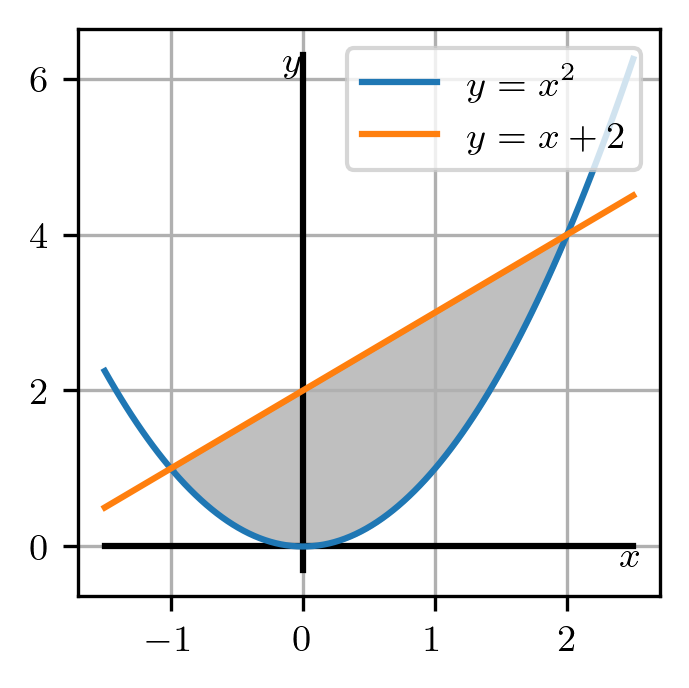
\includegraphics[width=3.75in]{./cap_progest/dados/fig_exer_entre_curvas/fig.png}
\end{figure}
\end{exer}
\begin{resp}

\begin{lstlisting}
print('P = (x,y)')
x = float(input('Digite o valor de x: '))
y = float(input('Digite o valor de y: '))

if x >= -1. and x <= 2 \
   and y >= x**2 and y <= x+2:
  print(f'P = ({x}, {y}) está entre as curvas.')
else:
  print(f'P = ({x}, {y}) não está entre as curvas.')
\end{lstlisting}

\end{resp}

\begin{exer}
  Considere um polinômio da forma
  \begin{equation}
    p(x) = (x-a)(bx^2 + cx + d).
  \end{equation}
  Desenvolva um código para a computação das raízes de $p(x)$, sendo os coeficientes $a$, $b$, $c$ e $d$ (números decimais) informados por usuária(o).
\end{exer}
\begin{resp}

\begin{lstlisting}
print('p(x) = (x-a)(bx^2 + cx + d)')
# entrada de dados
a = float(input('Digite o valor de a: '))
b = float(input('Digite o valor de b: '))
c = float(input('Digite o valor de c: '))
d = float(input('Digite o valor de d: '))

# cálculo das raízes
x1 = a
print(f'x1 = {x1}')
if b != 0.:
  delta = c**2 - 4*b*d
  x2 = (-c - delta**0.5)/(2*b)
  x3 = (-c + delta**0.5)/(2*b)
  print(f'x2 = {x2}')
  print(f'x3 = {x3}')
elif c != 0.:
  x2 = -d/c
  print(f'x2 = {x2}')
\end{lstlisting}

\end{resp}

\ifisbook
\newpage
\subsubsection{Respostas}
\shipoutAnswer
\fi


\section{Instruções de Repetição}\label{cap_progest_sec_repete}

\hl{Estruturas de repetição permitem a execução de um bloco de código várias vezes}. O número de vezes que o bloco é repetido pode depender de uma condição lógica (instrução {\PYTHONwhile}) ou do número de itens de um objeto iterável (instrução{\PYTHONfor}).

\subsection{Instrução \texttt{while}}

\hl{A instrução {\PYTHONwhile} permite a repetição condicional de um bloco de código}. Em {\python}, sua sintaxe é

\begin{lstlisting}
bloco_anterior
while condição:
  bloco
bloco_posterior
\end{lstlisting}

\begin{figure}[H]
  \centering
  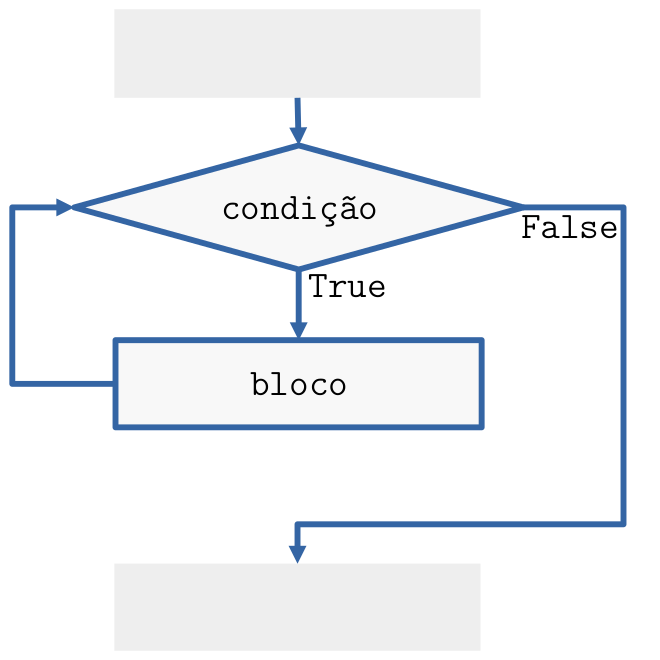
\includegraphics[width=2in]{./cap_progest/dados/fig_fg_while/fig.png}
  \caption{Fluxograma da estrutura de repetição {\PYTHONwhile}.}
  \label{fig:cap_progest_sec_repete:fig:fg_while}
\end{figure}

\begin{ex}\normalfont{(\hl{Somatório com \texttt{while}})}\label{cap_progest_ec_repete:ex:while_soma_num}
  O seguinte código, computa o \href{https://pt.wikipedia.org/wiki/Somat%C3%B3rio}{somatório}
  \begin{align}
    & s = \sum_{i=1}^{n}i \\
    & \text{}\quad = 1 + 2 + 3 + \cdots + n.
  \end{align}

\begin{lstlisting}
n = int(input('Digite um número natural n:\n'))

soma = 0
i = 1
while i <= n:
  soma = soma + i
  i = i + 1

print(f'1 + ... + {n} = {soma}')
\end{lstlisting}

\end{ex}

\begin{ex}\normalfont{\hl{(Aproximando a $\sqrt{x}$.)}}\label{cap_progest_sec_repete:ex:heron}
  O \href{https://en.wikipedia.org/wiki/Methods_of_computing_square_roots#Heron's_method}{método de Heron}{\heron} é um algoritmo para o cálculo aproximado da raiz quadrada de um dado número $x$, i.e. $\sqrt{x}$. Consiste na iteração\endnote{Aqui, assumimos a aproximação inicial $s^{(0)} = 1$, mas qualquer outro número não negativo pode ser usado.}
  \begin{align}
    & r^{(0)} = 1, \\
    & r^{(k+1)} = \frac{1}{2}\left(r^{(k)} + \frac{x}{r^{(k)}}\right),
  \end{align}
  para $k=0,1,2,\ldots,n-1$, onde $n$ é o número de iterações calculadas. Para $x\geq 0$ fornecido por usuária(o), o seguinte código computa a aproximação $r^{(5)}\approx \sqrt{x}$.

\begin{lstlisting}
x = float(input('Digite um número não negativo para x:\n'))
r = 1
k = 0
print(f'{k}: {r}')
while k < 5:
  r = 0.5*(r + x/r)
  k = k + 1
  print(f'{k}: {r}')
print(f'sqrt({x}) = {r}')
\end{lstlisting}

\end{ex}

\subsubsection{\texttt{break}}

\hl{A instrução {\PYTHONbreak} permite interromper um bloco de repetição e sair dele no momento em que ela é alcançada}.

\begin{ex}\label{cap_progest_sec_repete:ex:heron_break}
  No Exemplo \ref{cap_progest_sec_repete:ex:heron}, podemos observar que as aproximações $s^{(k)}\approx \sqrt{x}$ vão se tornando muito próximas umas das outras conforme as iterações convergem. Dessa observação, faz sentido que interrompamos as computações no momento em que a $k+1$-ésima iterada satisfaça
  \begin{equation}
    \left|r^{(k+1)}-r^{(k)}\right| < \texttt{tol}
  \end{equation}
  para alguma tolerância \lstinline+tol+ desejada.

\begin{lstlisting}
max_iter = 50
tol = 1e-15

x = float(input('Digite um número não negativo para x:\n'))

r0 = 1
k = 0
print(f'{k}: {r}')
while k < max_iter:
  k = k + 1
  r = 0.5*(r0 + x/r0)
  print(f'{k}: {r}')
  if (abs(r-r0) < tol):
    break
  r0 = r
print(f'sqrt({x}) = {r}')
\end{lstlisting}

\end{ex}

\subsection{Instrução \texttt{for}}

\hl{A instrução {\PYTHONfor} permite a iteração de um bloco de código para todos os itens de um dado objeto} (iterável). Em {\python}, sua sintaxe é

\begin{lstlisting}
bloco_anterior
for x in Iterável:
  bloco
bloco_posterior
\end{lstlisting}

Pode-se percorrer qualquer objeto iterável ({\PYTHONset}, {\PYTHONtuple}, {\PYTHONlist}, {\PYTHONdict}, etc.). \hl{Em cada iteração, o índice \texttt{x} toma um novo item do objeto. A repetição termina quando todos os itens do objeto tiverem sido escolhidos}. No caso de iteráveis ordenados ({\PYTHONtuple}, {\PYTHONlist}, {\PYTHONdict}, etc.), os itens são iterados na mesma ordem em que estão alocados no objeto.

\begin{ex}\label{cap_progest_sec_repete:ex:media_for}
  O seguinte código, computa a média aritmética do conjunto de números
  \begin{equation}
    A = \{1, 3, 5, 7, 9\}.
  \end{equation}

\begin{lstlisting}
soma = 0
for x in {1,3,5,7,9}:
  soma = soma + x
media = soma/5
print(f'média = {media}')
\end{lstlisting}

\end{ex}

\subsubsection{\texttt{range}}

\hl{A função {\PYTHONrange}([start], stop, [step]), retorna uma sequência iterável de números inteiros}, com início em \lstinline+start+ (padrão \lstinline+start=0+), passo \lstinline+step+ (padrão \lstinline+step=1+) e limite em \lstinline+stop+.

\begin{ex}
  Estudamos os seguinte casos:
  \begin{enumerate}[a)]
  \item Imprime, em ordem crescente, os primeiros $11$ números naturais.

\begin{lstlisting}[xrightmargin=2.5em]
for i in range(11):
  print(i)
\end{lstlisting}

\item Imprime, em ordem crescente, os números naturais contidos de $3$ a $13$, inclusive.

\begin{lstlisting}[xrightmargin=2.5em]
for i in range(3,14):
  print(i)
\end{lstlisting}

\item Imprime, em ordem crescente, os números naturais ímpares contidos de $3$ a $13$, inclusive.

\begin{lstlisting}[xrightmargin=2.5em]
for i in range(3,14,2):
  print(i)
\end{lstlisting}

\item Imprime, em ordem decrescente, os números naturais contidos de $3$ a $13$, inclusive.

\begin{lstlisting}[xrightmargin=2.5em]
for i in range(13,2,-1):
  print(i)
\end{lstlisting}

\end{enumerate}

\end{ex}

\begin{ex}\normalfont{(\hl{Somatório com \texttt{for}}.)}\label{cap_progest_ec_repete:ex:for_soma_num}
  No Exemplo \ref{cap_progest_ec_repete:ex:while_soma_num}, computados
  \begin{equation}
    s = \sum_{i=1}^n i
  \end{equation}
  usando um laço {\PYTHONwhile}. Aqui, apresentamos uma nova versão do código com a instrução {\PYTHONfor}.

\begin{lstlisting}
n = int(input('Digite um número natural n:\n'))
soma = 0
for i in range(1,n+1):
  soma = soma + i
print(f'1 + ... + {n} = {soma}')
\end{lstlisting}

\end{ex}

\begin{ex}
  No Exemplo \ref{cap_progest_sec_repete:ex:heron_break}, apresentamos um código para o cálculo aproximado de $\sqrt{x}$ pelo Método de Heron. Aqui, temos uma nova versão com a instrução {\PYTHONfor} no lugar do laço {\PYTHONwhile}.

\begin{lstlisting}
max_iter = 50
tol = 1e-15

x = float(input('Digite um número não negativo para x:\n'))

r0 = 1
k = 0
print(f'{k}: {r}')
for k in range(max_iter):
  r = 0.5*(r0 + x/r0)
  print(f'{k+1}: {r}')
  if (abs(r-r0) < tol):
    break
  r0 = r
print(f'sqrt({x}) = {r}')
\end{lstlisting}

\end{ex}

\subsection{Exercícios}

% exercícios de compreensão

\begin{exer}
  Complete as lacunas.
  \begin{enumerate}[a)]
    % a)
    \item Intruções de \underline{\phantom{repetição}} permitem a execução de um bloco de código várias vezes.
    % b)
    \item A instrução \underline{\phantom{{\PYTHONwhile}}} permite a repetição de um bloco de código com base em uma condição lógica.
    % c)
    \item A instrução {\PYTHONfor} permite a repetição \underline{\phantom{iterada}} de um bloco de código.
  \end{enumerate}
\end{exer}
\begin{resp}
  a) repetição; b) {\PYTHONwhile}; c) iterada.
\end{resp}

% exercícios de programação

\begin{exer}
  Faça o fluxograma do código apresentado no Exemplo \ref{cap_progest_ec_repete:ex:while_soma_num}. Também, desenvolva uma versão melhorada do código, que verifica se o valor de $n$ digitado pela(o) usuária(o) é não negativa. Caso afirmativo, computa o somatório, noutro caso apenas imprime mensagem de que o $n$ deve ser não negativo.
\end{exer}
\begin{resp}

\begin{lstlisting}
n = int(input('Digite um número natural n:\n'))
if (n >= 0):
  soma = 0
  i = 1
  while (i <= n):
    soma = soma + i
    i = i + 1

  print(f'1 + ... + {n} = {soma}')
else:
  print('ERRO: n deve ser não negativo.')
\end{lstlisting}

\end{resp}

\begin{exer}
  Faça um fluxograma para o código apresentado no Exemplo \ref{cap_progest_sec_repete:ex:media_for}.
\end{exer}
\begin{resp}
  Dica: consulte o fluxograma apresentado no Exemplo \ref{cap_progest_sec_est:ex:for}.
\end{resp}

\begin{exer}
  Crie um objeto do tipo {\PYTHONrange} para cada uma das seguintes sequências:
  \begin{enumerate}
  \item Sequência crescente de todos os números inteiros de $0$ até $99$, inclusive.
  \item Sequência crescente de todos os números pares de $-5$ até $15$.
  \item Sequência decrescente de todos os números de $100$ a $0$, inclusive.
  \item Sequência decrescente de todos os números múltiplos de $3$ entre $17$ e $-3$.
  \end{enumerate}
\end{exer}
\begin{resp}
  \begin{enumerate}[a)]
  \item \lstinline+range(100)+
  \item \lstinline+range(-4,15,2)+
  \item \lstinline+range(100,-1,-1)+
  \item \lstinline+range(15,-4,-3)+
  \end{enumerate}
\end{resp}

\begin{exer}
  Considere o somatório entre dois números inteiros $n \leq m$
  \begin{align}
    & s = \sum_{i=n}^m i \\
    & \text{}\quad = n + (n+1) + (n+2) + \cdots + m
  \end{align}
  Com números informados pela(o) usuária(o), escreva duas versões de códigos para a computação desse somatório:
  \begin{enumerate}[a)]
  \item Usando a instrução {\PYTHONwhile}.
  \item Usando a instrução {\PYTHONfor}.
  \end{enumerate}
\end{exer}
\begin{resp}
a)

\begin{lstlisting}
n = int(input('Digite um número inteiro n:\n'))
m = int(input('Digite um número inteiro m>n:\n'))
soma = 0
i = n
while (i<=m):
  soma = soma + i
  i = i + 1
print(f'n+...+m = {soma}')
\end{lstlisting}

b)

\begin{lstlisting}
n = int(input('Digite um número inteiro n:\n'))
m = int(input('Digite um número inteiro m>n:\n'))
soma = 0
for i in range(n,m+1):
  soma = soma + i
print(f'n+...+m = {soma}')
\end{lstlisting}

\end{resp}

\begin{exer}
  A \href{https://pt.wikipedia.org/wiki/S\%C3\%A9rie_harm\%C3\%B3nica_(matem\%C3\%A1tica)}{série harmônica} é
  \begin{equation}
    \sum_{k=1}^\infty \frac{1}{k} = 1 + \frac{1}{2} + \frac{1}{3} + \cdots + \frac{1}{n} + \cdots
  \end{equation}
  Com $n$ fornecido por usuária(o), crie códigos que computem o valor da soma harmônica
  \begin{equation}
    s = \sum_{k=1}^n \frac{1}{k} = 1 + \frac{1}{2} + \frac{1}{3} + \cdots + \frac{1}{n}.
  \end{equation}
  \begin{enumerate}[a)]
  \item Use uma estrutura de repetição {\PYTHONwhile}.
  \item Use uma estrutura de repetição {\PYTHONfor}.
  \end{enumerate}
\end{exer}
\begin{resp}
a)

\begin{lstlisting}
n = int(input('Digite um número natural n:\n'))
s = 0
k = 1
while (k <= n):
  s = s + 1/k
  k = k + 1
print(s)
\end{lstlisting}

b)

\begin{lstlisting}
n = int(input('Digite um número natural n:\n'))
s = 0
for k in range(n):
  s = s + 1/(k+1)
print(s)
\end{lstlisting}

\end{resp}

\begin{exer}
  O cálculo do logaritmo natural pode ser feito pela seguinte série de potências
  \begin{equation}
    \ln(1 + x) = \sum_{k=1}^\infty (-1)^{k+1}\frac{x^k}{k}
  \end{equation}
  Desenvolva um código que compute a aproximação do $ln(2)$ dada por
  \begin{equation}
    \ln(2) = \sum_{k=1}^n \frac{(-1)^{k+1}}{k}
  \end{equation}
  com $n >= 1$ número inteiro fornecido por usuária(o).
  \begin{enumerate}[a)]
  \item Use uma estrutura de repetição \verb+while+.
  \item Use uma estrutura de repetição \verb+for+.
  \end{enumerate}
\end{exer}
\begin{resp}
  a)

\begin{lstlisting}
n = int(input('Digite um número natural n >= 1: '))

s = 0
k = 1
while (k <= n):
  s += (-1)**(k+1)/k
  k += 1
print(f'ln(2) aprrox. {s}')
\end{lstlisting}

b)

\begin{lstlisting}
n = int(input('Digite um número natural n >= 1: '))

s = 0
for k in range(1, n+1):
  s += (-1)**(k+1)/k
  k += 1
print(f'ln(2) aprrox. {s}')
\end{lstlisting}

\end{resp}

\begin{exer}
  O \href{https://pt.wikipedia.org/wiki/Fatorial}{fatorial} de um número natural é definido pelo \href{https://pt.wikipedia.org/wiki/Produt\%C3\%B3rio}{produtório}
  \begin{align}
    & n! := \prod_{k=1}^{n}k \\
    & \text{}\quad = 1\cdot 2\cdot 3 \cdot (n-1)\cdot n
  \end{align}
  e $0! := 1$. Com $n$ informado por usuária(o), crie códigos para computar $n!$ usando:
  \begin{enumerate}[a)]
  \item uma estrutura de repetição {\PYTHONwhile}.
  \item uma estrutura de repetição {\PYTHONfor}.
  \end{enumerate}
\end{exer}
\begin{resp}
  a)

\begin{lstlisting}
n = int(input('Digite um número natural n:\n'))
fat = 1
k = 1
while (k < n):
  k = k + 1
  fat = fat * k
print(f'{n}! = {fat}')
\end{lstlisting}

b)

\begin{lstlisting}
n = int(input('Digite um número natural n:\n'))
fat = 1
for k in range(1,n+1):
  fat = fat * k
print(f'{n}! = {fat}')
\end{lstlisting}

\end{resp}

\begin{exer}
  O \href{https://pt.wikipedia.org/wiki/E_(constante_matem\%C3\%A1tica)}{número de Euler}{\euler} é tal que
  \begin{align}
    & e := \sum_{k=0}^\infty \frac{1}{n!} \\
    & \text{}\quad = \frac{1}{0!} + \frac{1}{1!} + \frac{1}{2!} + \cdots + \frac{1}{n!} + \cdots
  \end{align}
  Com $n$ fornecido por usuária(o), desenvolva um código que computa a aproximação
  \begin{equation}
    e \approx e^{(n)} = \sum_{k=0}^n \frac{1}{n!}.
  \end{equation}
  Qual o número $n$ tal que $\left|e^{(n)} - e^{(n-1)}\right|<10^{-15}$?
\end{exer}
\begin{resp}

\begin{lstlisting}
n = int(input('Digite um número natural n:\n'))
fat = 1
e = 1
for k in range(1,n+1):
  fat = fat * k
  e = e + 1/fat
print(f'e = {e}')
\end{lstlisting}

\end{resp}

\begin{exer}
  Com $n\geq 1$ número natural fornecido por usuária(o), crie um código que verifique se $n$ é um \href{https://pt.wikipedia.org/wiki/N\%C3\%BAmero_primo}{número primo}.
\end{exer}
\begin{resp}

\begin{lstlisting}
n = int(input('Digite um número natural n>=1:\n'))
primo = True
for i in range(2, n//2+1):
  if (n % i == 0):
    primo = False
    break
print(f'{n} é primo? {primo}')
\end{lstlisting}

\end{resp}

\ifisbook
\subsubsection{Respostas}
\shipoutAnswer
\fi
